%%
%  ******************************************************************************
%  * #file    Szablon_raportu_EN_Latex.tex
%  * #author  Adrian Wójcik   adrian.wojcik(at)put.poznan.pl
%  *          
%  * #commit  Patryk Kościk   koscikpatryk(at)gmail.com
%  *          Modified the template for Projekt przejsciowy purposes          
%  *          
%  * #version 1.0
%  * #date    09-Mar-2022
%  * #brief   PROJPRZEJ
%  *
%  ******************************************************************************
%%  
\documentclass[11pt, a4paper]{article}

\usepackage{RAPORT_LASER_PP}

% Wypełnijcie te dyrektywy zgodnie z waszym tematem
% \lab      -> NAZWA CZUJNIKA, np.: 'DHT22'
% \comment  -> Króciutki opis co to, np.: 'Cyfrowy budżetowy czujnik temperatury'
%
\lab{Dioda laserowa}
\comment{Moduł diody laserowej}
\author{Adam Rewekant}

% Absolutny zakaz dotykania tego tutaj bo jak dotkiecie to coś jebnie
\university{Politechnika Poznańska}
\faculty{Wydział Automatyki, Robotyki i Elektrotechniki}
\institute{Instytut Robotyki i Inteligencji Maszynowej}
\department{Zakład Sterowania i Elektroniki Przemysłowej}
\addbibresource{bib/Laser.bib}
\nocite{*}

%%
%
% Początek dokumentu
%
%%
\begin{document}

%% Strona tytułowa %%
\mainpage{{fig/laser/ModulLaser}}

\newpage
\section*{Opis elementu} \addcontentsline{toc}{section}{Wstęp}
Moduł lasera KY-008 składa się z diody laserowej oraz trzech pinów. Dwa piny odpowiedzialne są za zasilanie (5V oraz GND), a trzeci pin jest pinem sygnałowym. Po podaniu na niego stanu wysokiego, laser zaczyna świecić.

\vspace{0.5cm}
\begin{figure}[h]
\centering
\begin{subfigure}{.5\textwidth}
  \centering
  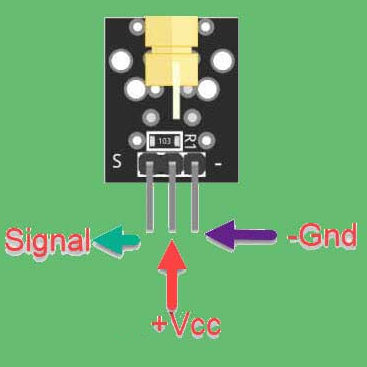
\includegraphics[width=.4\linewidth]{fig/laser/zdjecie1.png}
  \caption{Moduł KY-008 \cite{zdjecia}}
  \label{fig:sub1}
\end{subfigure}%
\begin{subfigure}{.5\textwidth}
  \centering
  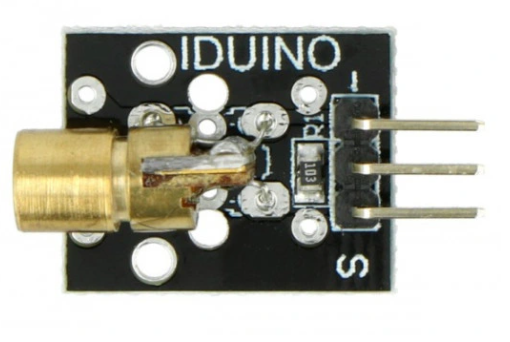
\includegraphics[width=.6\linewidth]{fig/laser/zdjecie2.png}
  \caption{Moduł KY-008 \cite{budowa}}
  \label{fig:sub2}
\end{subfigure}
\caption{Przykładowe zdjęcia modułu lasera.}
\label{fig:test}
\end{figure}
\vspace{0.5cm}

Laser to moduł zawierający diodę, która emituje światło. Podobnie jak inne diody, jest ona wykonana z materiałów półprzewodnikowych pn.


\vspace{0.5cm}
\begin{figure}[h]
\centering
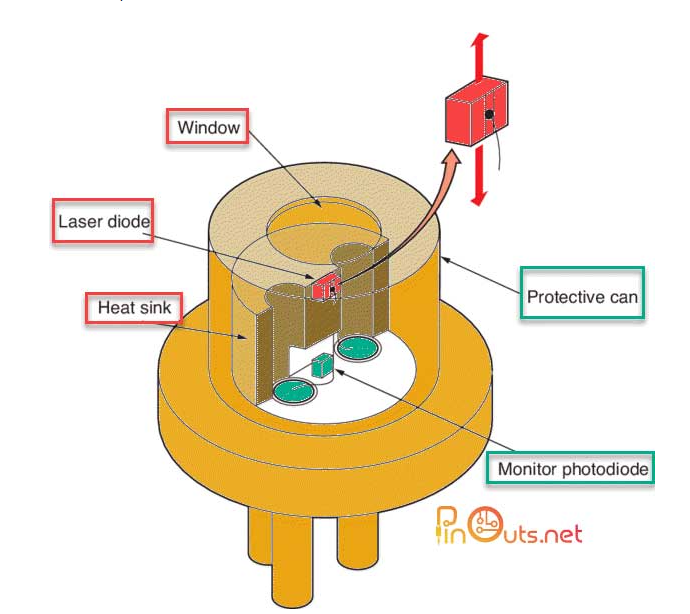
\includegraphics[width=.75\linewidth]{fig/laser/budowa.png}
\caption{Budowa lasera.\cite{budowa}}
\label{fig:test}
\end{figure}
\vspace{0.5cm}

\newpage
\section{Użycie czujnika}

\vspace{0.5cm}
\begin{figure}[h!]
    \centering
    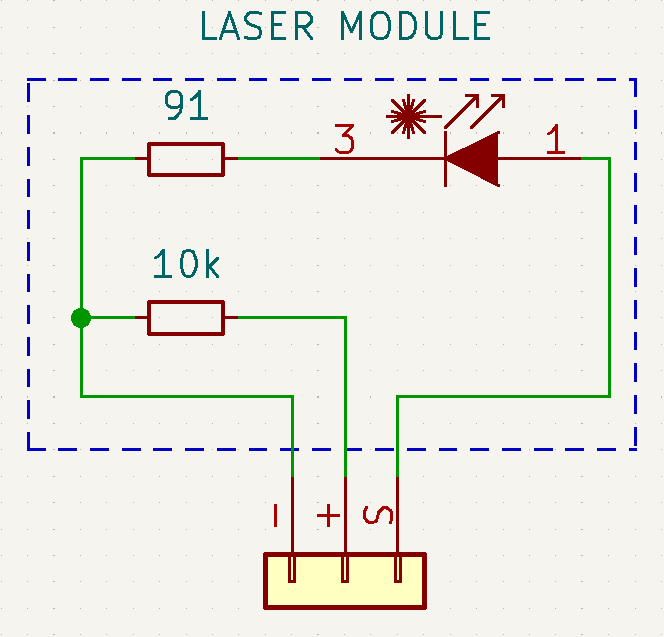
\includegraphics[width=6cm]{fig/laser/kicadLaser.png}
    \caption{Połaczenie elektryczne}
    \label{fig:my_label}
\end{figure}
\vspace{0.5cm}

Doskonałym zastosowaniem modułu laserowego jest komunikacja szeregowa za pomocą światła laserowego. Informacje są przesyłane przez światło bez żadnych czynników środowiskowych. Rolę odbiornika może pełnić fotodioda.

\section{Prezentacja działania układu}

\vspace{0.5cm}
\begin{figure}[h!]
    \centering
    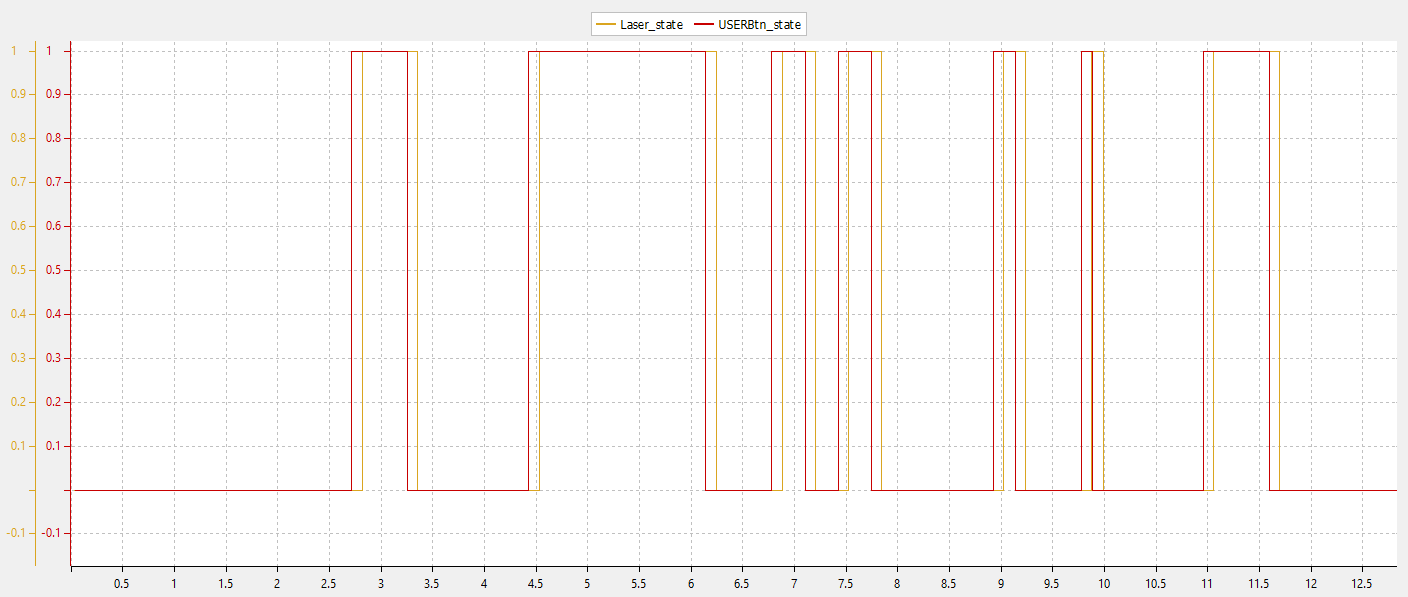
\includegraphics[width=1\textwidth]{fig/laser/SWV.png}
    \caption{Przedstawienie działania układu na wykresie.}
    \label{fig:my_label}
\end{figure}

Jak widać po wciśnięciu przycisku (USERBtn\_state) na wejściu lasera (Laser\_state) pojawia się stan wysoki co powoduje jego świecenie (wprowadzone zostało opóźnienie w celu lepszego przedstawienia działania układu).

\newpage

\vspace{0.5cm}
\begin{figure}[h!]
    \centering
    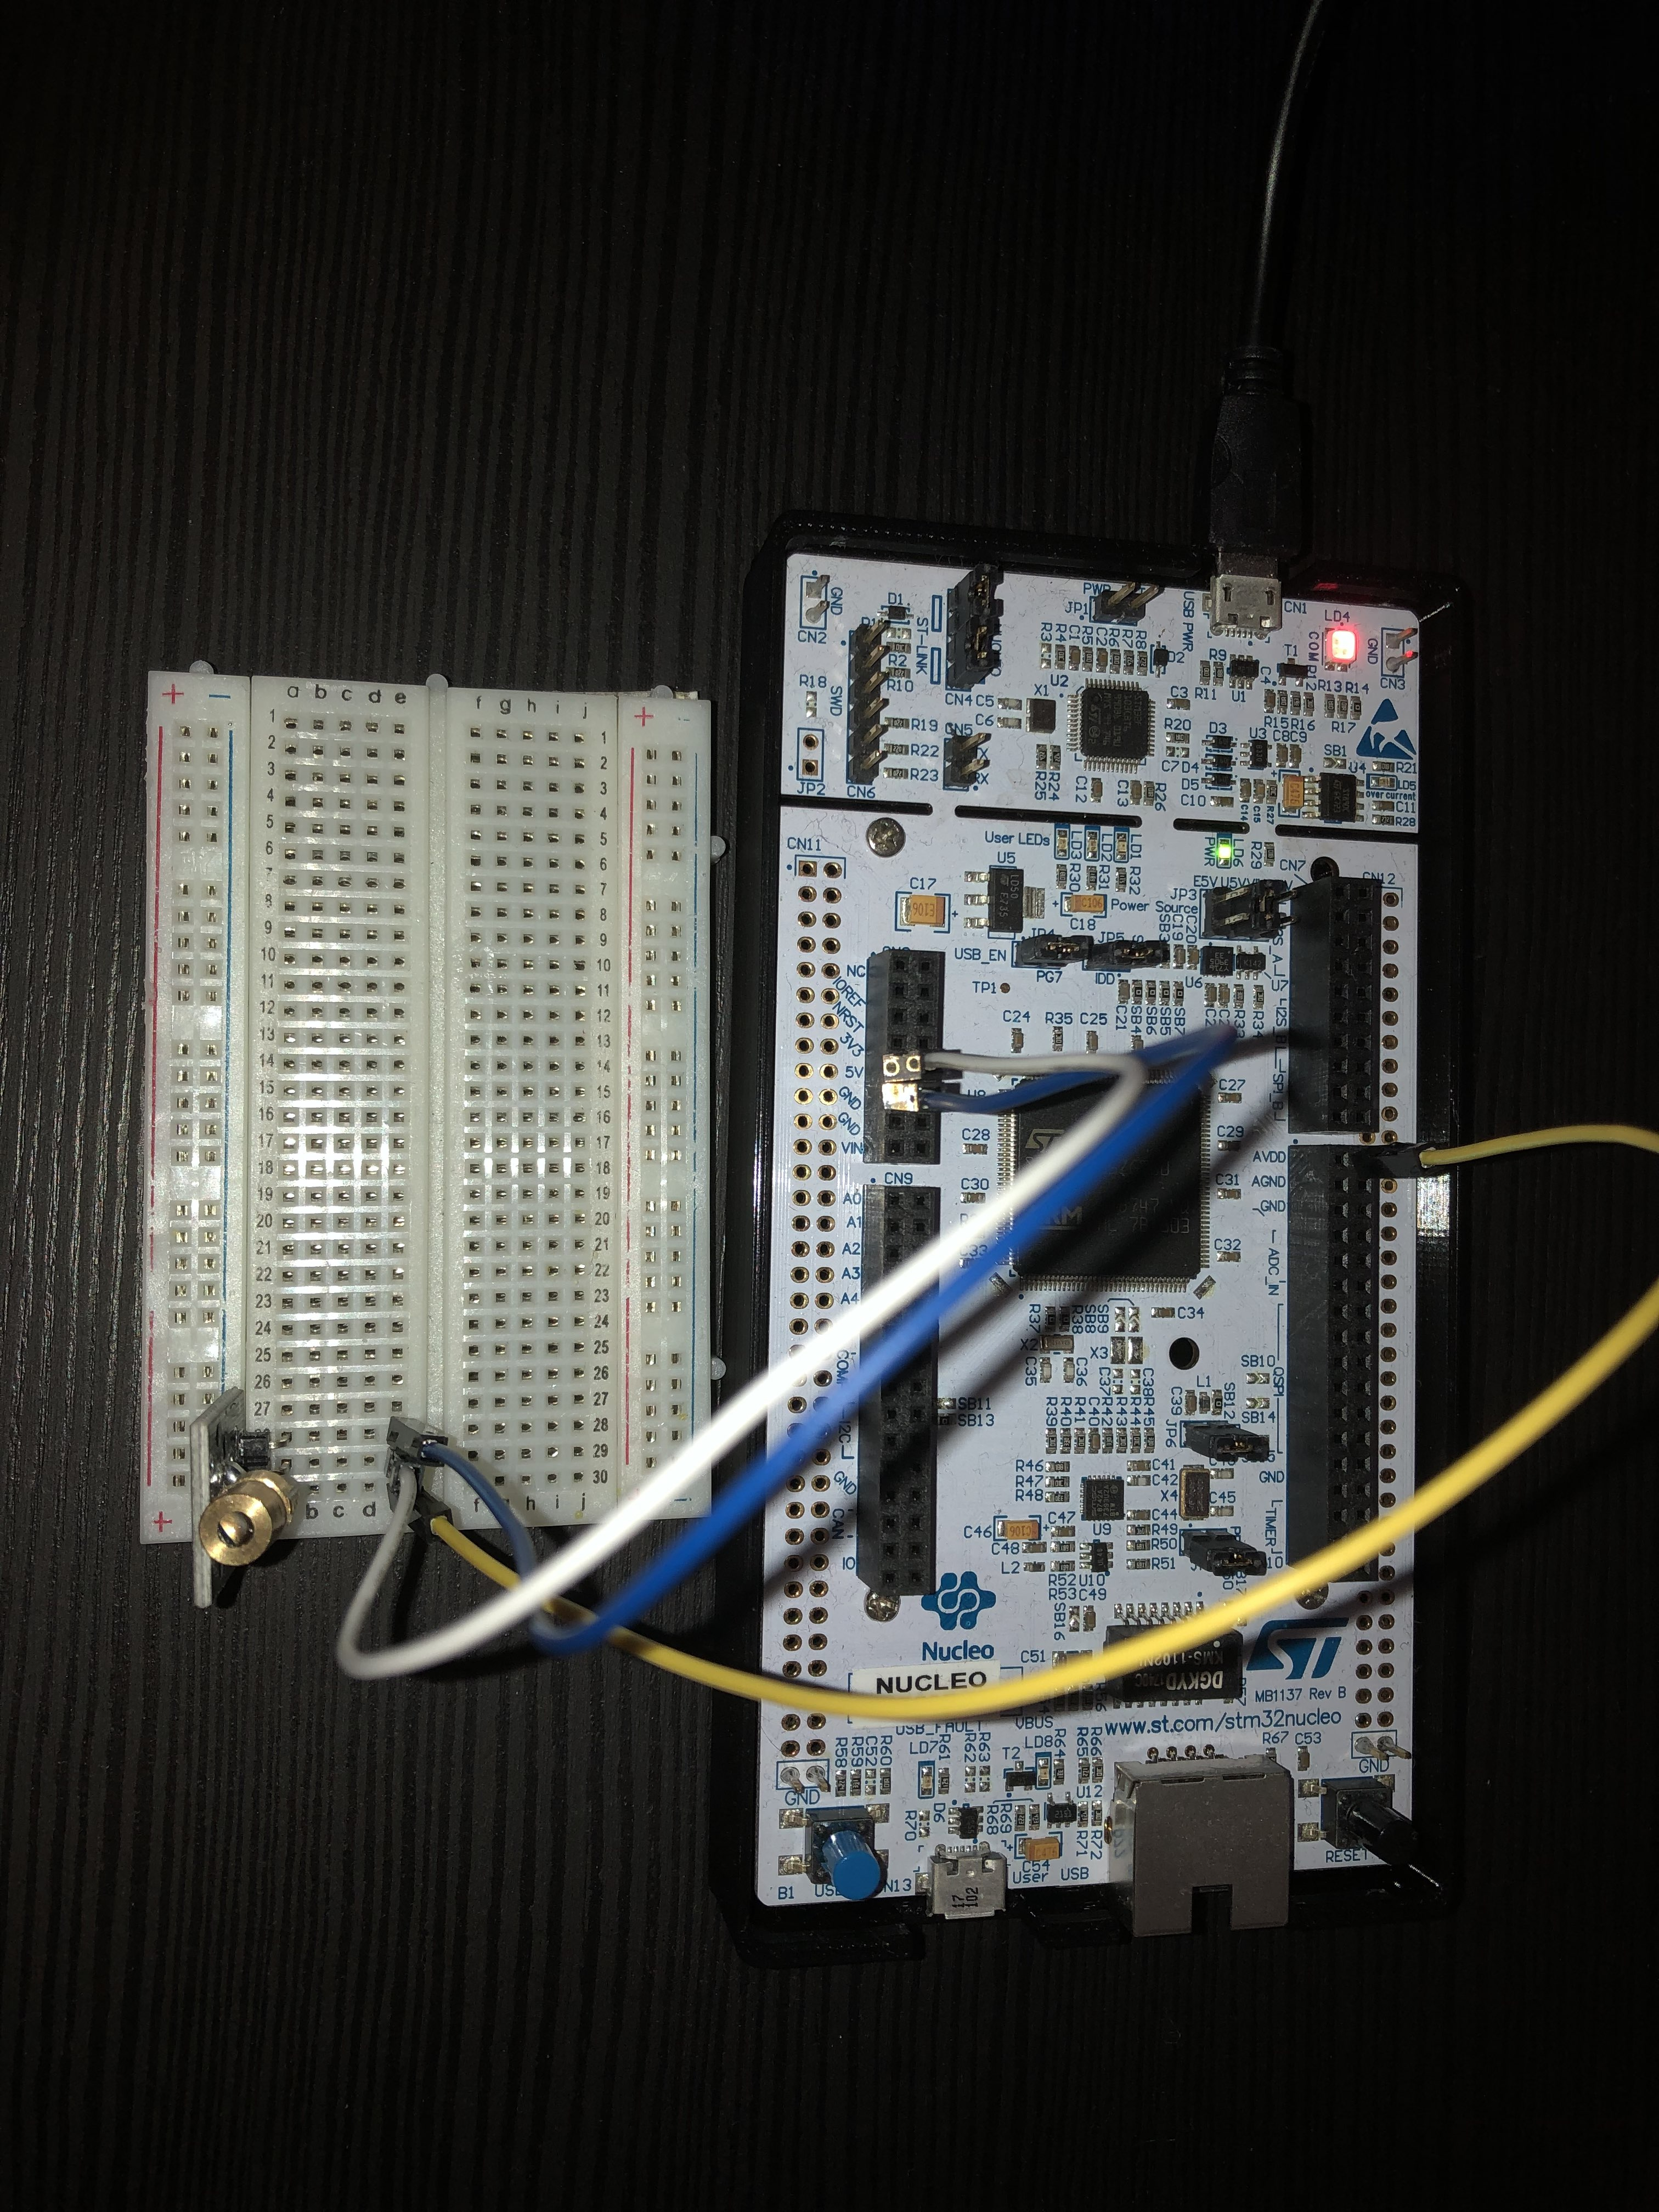
\includegraphics[width=1\textwidth]{fig/laser/zdjecieukladu.png}
    \caption{Zdjęcie układu.}
    \label{fig:my_label}
\end{figure}

Działanie układu zostało jeszcze zaprezentowane na krótkim wideo \cite{youtube}.

\printbibliography[heading=bibintoc]

\end{document}
